\section{Chapter 8 - Semiconductor Crystals} 

		\begin{description}
			\item[Semiconductor:] $10^{-2}$ - $10^{9}$ ohm-cm at RT
			\item[Insulator:] $10^{14}$ ohm at T=0K
			\item[Intrinsic temperature range:]  Range of temperature where the electrical properties are not affected by impurities in the crystal.
		\end{description}
		
		\subsection{Band Gap}
			Intrinsic conductivity $\sigma$ and intrinsic carrier concentration $n$ are controlled by $\frac{E_g}{k_BT}$.  $\frac{E_g}{k_BT}>>1\Rightarrow n , \sigma << 1$, $\frac{E_g}{k_BT}<<1\Rightarrow n , \sigma >> 1$.
			
			\begin{description}
				\item[Direct band gap:] ~\\
									$\textbf{k}(photon) = \textbf{k}_c $ ??\\
										$\Rightarrow E_g = \hbar \omega$
				\item[Indirect band gap:]  ~\\
										 $\textbf{k}(photon) = \textbf{k}_c + \textbf{K}\approx  0$ \\
										Emitted phonon: $\textbf{K}=-\textbf{k}_g \Rightarrow \hbar \omega = E_g  + \hbar \Omega$ \\
										Absorbed phonon: $\textbf{K}=\textbf{k}_g \Rightarrow \hbar \omega = E_g  - \hbar \Omega$ \\
			\end{description}
			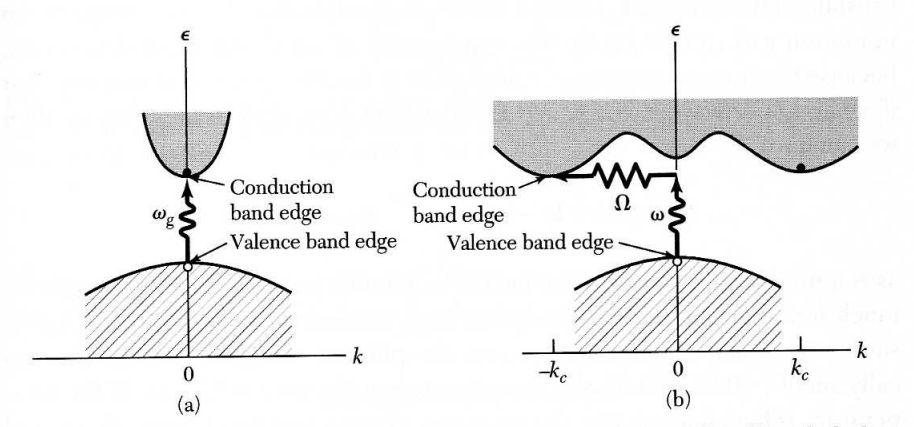
\includegraphics[scale=0.6]{direct_indirect.png}
			~\\
			
		\subsection{Equations of Motion}
				The motion of a wavefunction in an applied electric field.   Wavepacket made up of wavefunctions assembled near a wavevector \textit{k}.  The group velocity is:
				\begin{equation}
					v_g = \frac{d\omega}{dk}
				\end{equation}
			The frequency associated with a wavefunction of energy $\boldsymbol{\epsilon}$ is $\omega = \frac{\boldsymbol{\epsilon}}{\hbar}$  Therefore:
				\begin{equation}
					v_g = \frac{1}{\hbar}\frac{d\boldsymbol{\epsilon}}{dk}
				\end{equation}
				\begin{equation}
					\textrm{\textbf{v}} = \frac{1}{\hbar} \nabla_{\boldsymbol{k}} \boldsymbol{\epsilon}(\boldsymbol{k})
				\end{equation}
				This can be used to show that an external force on an electron can be related to the change in wave vector:
				\begin{equation}
					\hbar \frac{d\textrm{\textbf{k}}}{dt} = \textrm{\textbf{F}}
				\end{equation}
				The force term includes the Lorentz force so:
				\begin{equation}
					\hbar \frac{d\textrm{\textbf{k}}}{dt} = -e\textrm{\textbf{v}} \times \textrm{\textbf{B}}
				\end{equation}
				exchanging for the group velocity we have:
				\begin{equation}
					\hbar \frac{d\textrm{\textbf{k}}}{dt} = -e\frac{1}{\hbar^2} \nabla_{\boldsymbol{k}} \boldsymbol{\epsilon}(\boldsymbol{k}) \times \textrm{\textbf{B}}
				\end{equation}
				
				Which shows that electrons move along constant energy surfaces normal to the direction of the \textbf{B} field in \textbf{k} space.
		
		\subsection{Holes}
			\begin{description}
				\item[1)] $\vect{k}_h$ = $-\vect{k}_e$
				\item[2)] $\boldsymbol{\epsilon}_h(\vect{k}_h)$ = $-\boldsymbol{\epsilon}_e(\vect{k}_e)$
				\item[3)] $\vect{v}_h$ = $-\vect{v}_e$
				\item[4)] $m_h$ = $-m_e$
				\item[5)] $\hbar\frac{d\vect{k}_e}{dt} = e(\vect{E} + \frac{1}{c}\vect{v}_h\times\vect{B})$
			\end{description}
		\subsection{Effective mass}
			With the free electron we notice the reciprocal effect mass $\frac{1}{m^*}$ determines the curvature of the band $\frac{d\boldsymbol{\epsilon}}{d\vect{k}}$ if we remember that:
			\begin{equation}
				\boldsymbol{\epsilon} = \frac{\hbar^2 \vect{k}^2}{2m^*}
			\end{equation}
			
			